\section{Sunquakes}
\subsection{Introduction}
%Chronological soft intro; use some of the lit review,
%making sure to emphasize the connection to solar flares;Look at early papers predicting sunquakes(Wolff 70s and Kosovichev and Zharkova);the importance of sunquakes


During this age of space-born solar astronomy, understanding the highly dynamic environment of the Sun's atmosphere is a study enriched by a wealth of high detail observations. With each newly launched space instrument the spatial resolution of collected data increases, which coupled with those spacecraft that are tailored to capture light of previously unobserved wavelengths, often leads to new phenomena being observed. Eruptive solar flares fall into this category, in that spacecraft have provided observations that challenge the current theoretical view that the standard eruptive flare model (CSHKP model: \citep{1964NASSP..50..451C, 1966Natur.211..695S, 1974SoPh...34..323H, 1976SoPh...50...85K} puts forward.

Solar flares are one of the most energetic events to occur in the Sun's atmosphere, where by stored magnetic energy is released in the form of heat, mass motions, and accelerated particles. This highly dynamic process produces many measurable signatures, such as emission from $\gamma$-ray to optical wavelengths, a high percentage of which agree with the CSHKP model. However, this is not the full picture. The standard flare model has been modified to include new observations many times over the years (e.g., \cite{2011LRSP....8....6S}) and is still unable to describe some observed phenomena. Therefore there is still work to be done before a true account of the complex nature of solar flares can be realised.

Sunquakes are an observable feature during some solar flares that the standard model is unable to explain. It is believed that they are the result of energy and momentum released during the flare impacting the lower solar atmosphere. During a solar flare, energy is released high up in the solar atmosphere and transported down to lower altitudes. If a sufficient amount of momentum impacts the lowest atmospheric layer, then acoustic waves are produced which propagate into sub-surface layers of the Sun and are then observed on the solar surface as a sunquake (see Figure \ref{sunquake-cartoon}a). As acoustic wave-fronts travel into the interior they encounter layers of increasing density causing refraction back toward the solar surface (see Figure \ref{sunquake-cartoon}b). At which point, waves can be observed as circular formations in the surface plasma, expanding outward from a point of origin (see Figure \ref{mdiquake96}).


\begin{figure}[hb]%\label{sunquake-cartoon}
  \begin{center}
  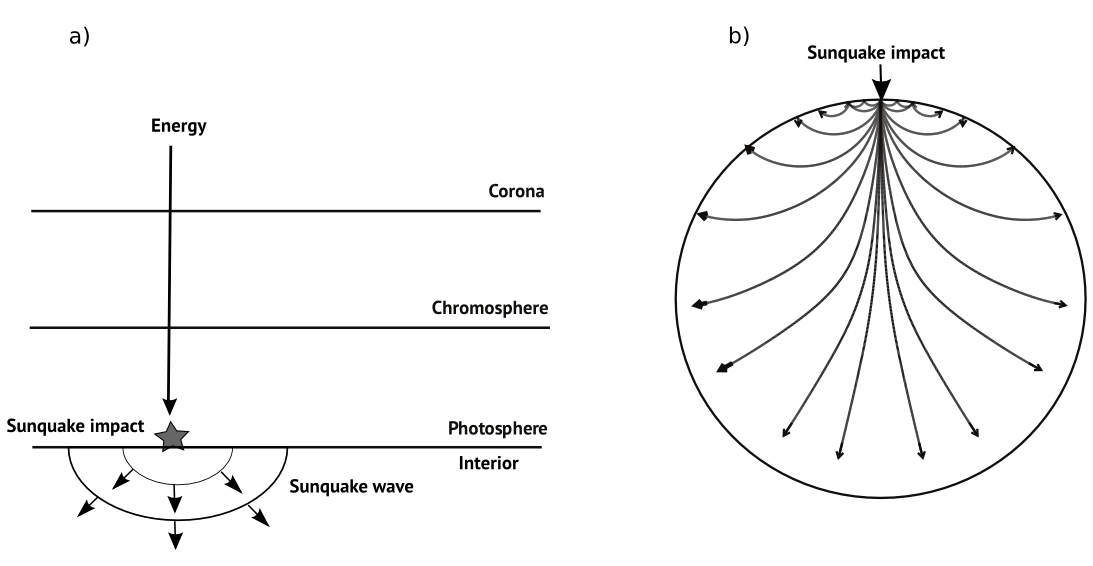
\includegraphics[width=0.99\textwidth]{sunquake-cartoon}
  \caption{Sunquake cartoon: a) Shows a basic picture of sunquake production. Energy moves down through the solar atmosphere impacting the photosphere and generating a sunquake. b) Shows acoustic wave-fronts propagating into the interior of the Sun. Wave-fronts refract back toward the surface as they encounter increasingly dense sub-surface layers. Waves reaching the surface disturb material in a pattern resembling ripples in a pond. Courtesy of \cite{2014arXiv1402.1249K}}\label{sunquake-cartoon}
\end{center}
\end{figure}

\subsection{Sunquake Observations}
The idea that solar flares can cause acoustic waves inside the Sun was originally put forward by \citep{1972ApJ...176..833W}. Wolff made the connection that a large solar flare releasing enough energy to heat the photosphere, would generate expansion of photospheric material, which could lead to an impulsive stimulation of oscillations in the Sun's interior. Wolff also commented that it would be difficult to observe interior oscillations with current (in the 1970s) solar velocity measurement techniques.

A little over twenty years later and Wolff's idea was built upon by \cite{1995ESASP.376b.341K}, who showed theoretically that acoustic waves in the solar interior could be generated by a large solar flare, and that they may be detectable. A year later and the first detection of a sunquake was made by \cite{1998Natur.393..317K} during an X class solar flare on July the 9th 1996. Their observational data came from the Solar and Heliospheric Observatory (SOHO) via the Michelson Doppler Imager (MDI) which images the movement of photospheric material by analysing shifts in wavelength of the emitted light. They observed a prominent impulsive downward signature in the Dopplergrams directly over a compact point source which subsequently emanates a set of concentric acoustic waves (see Figure \ref{mdiquake96}). The timing of maximum downward velocity of material derived from the Dopplergrams was out of sync with peak hard x-ray measurements by around a minute. This time delay, coupled with white-light enhancement in the lower atmosphere led to the conclusion that during the flare, accelerated energetic particles heat the cool dense chromosphere causing a shock front which travels downward, depositing energy in lower atmospheric layers, generating a sunquake.

\begin{figure}[hb]
  \begin{center}
  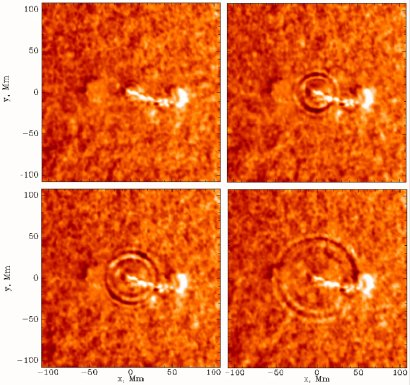
\includegraphics[width=0.80\textwidth]{soho-mdi-quake-96}
\caption{\cite{1998Natur.393..317K} produced SOHO MDI Dopplergrams from the 1996 July 9th, X class solar flare showing the sunquake expanding outward from it's seismic epicentre to a radial distance of $1.2\times10^{8}$ metres. Wave-fronts accelerate from a velocity of 30km/s to 100km/s}\label{mdiquake96}
\end{center}
\end{figure}


The first sunquake observation opened up a whole new area of solar physics, leading to subsequent detections associated other flares. The majority of observations show that sunquakes are often the product of highly impulsive flares, with the acoustic source aligning spatially with white light enhancement in the lower solar atmosphere and hard x-ray emission in the upper-atmosphere \citep{2005ApJ...630.1168D, 2007ApJ...664..573Z}. \cite{2005ApJ...630.1168D} went on to calculate the energy needed to stimulate the propagation of an acoustic wave in the sub-photosphere, finding that only $\sim10^{-3}$ of the energy released by a flare is enough to generate a sunquake. This was an important calculation because it forced the solar community to consider that it might be possible for low energy flares to produce sunquakes, leading to subsequent work by \cite{2008SoPh..251..613M} looking at seismicity of M-class flares.

A paper by \cite{2000ApJ...531L..75H} put forward for the first time, that sunquake production may depend on the changing configuration of the local magnetic field. This idea was further reinforced by \cite{2001ApJ...550L.105K} reporting observations of impulsive changes in magnetic field strength at the photosphere during a solar flare. These magnetic transients were shown to approximately correlate in time and space with hard x-rays, impulsive increases in plasma velocity and increased emission. This line of study was continued \citep{2009MNRAS.395L..39M}, investigating the magnetic field variation of the photosphere in many flares. The study found that some flares with seismicity do not have a spatial and temporal correlation between sunquakes and magnetic transients. Some flares have magnetic transients and no seismicity, and some flares have a good co-spatial alignment of acoustic activity and magnetic variability. It was noted that the impulsiveness of the magnetic field variation could be important as to whether a sunquake is generated.

Some of the most intriguing of sunquake observations are those that do not abide by the usual set of observable features, in that they are not necessarily associated with hard x-rays and excess white-light emission. For example, a statistical survey carried out by \cite{2012SoPh..277..317P}, highlighted a flare containing three footpoints with a seismic source that was co-temporal but not co-spatial with it's closest HXR footpoint; and another source which was co-spatial and co-temporal with its nearest HXR footpoint. This showed that a sunquake does not necessarily correlate with locations of peak emission. Another example by \cite{2011ApJ...741L..35Z} reports an observation of two seismic sources associated with footpoints of an erupting flux rope. During the eruption, the magnetic field above each seismic source undergoes an abrupt permanent reconfiguration. The authors cite the possibility that there exists particle beams low enough in population that HXR emission is undetectable. Further papers investigating the same event \citep{2013SoPh..284..315Z} show that there are downward motions of material above the seismic sources and that energy provided by magnetic transients may not be able to account for the acoustic power generated. These observational oddities prove that mechanisms that generate sunquakes are not well understood and there is much research to be done to classify the different progenitors.

\subsubsection{Sunquake Progenitors}\label{sunprog}
%list and explain current theories of sunquake generation
%making sure to highlight the different observables that can identify each mechanism, eg wlf = evidence of radiative backwarming


The progenitors of sunquakes are still unknown and as a result this is an exciting area of research with discoveries still to be made. The general consensus, in terms of valid mechanisms that could cause this phenomenon is an area of contention, however the following progenitors are thought to be at least partly responsible. \\

\begin{itemize}
\item \textbf{Radiative backwarming} as a mechanism for producing sunquakes, was first put forward by \cite{2005ApJ...630.1168D} to account for a spatial correlation between seismic sources and white light emission from the lower atmosphere. During a solar flare, high energy electrons and photons impulsively heat the lower chromosphere or photosphere producing an enhancement in white light emission \citep{1989SoPh..124..303M}. This causes an impulsive increase in radiation pressure and gas pressure exerted on the photosphere, generating acoustic waves which propagate into the sub-photosphere. \\

\item \textbf{Sudden magnetic field reconfiguration} was first detailed by \cite{2008ASPC..383..221H}. Solar flares are violent physical processes dictated by the interplay between reconnecting magnetic fields and charged solar plasma.
If the magnetic field close to the photosphere relaxes to a more horizontal alignment it can impart a Lorentz force on the local plasma environment, resulting in the production of acoustic waves in the sub-photosphere. The key parameter for this mechanism seems to be that the field has to reconfigure in an sufficiently impulsive manner to generate enough force to induce seismic waves. \\

\item \textbf{Shocks} are a mechanism originally proposed in initial work by \cite{1995ESASP.376b.341K} and \cite{1998Natur.393..317K}, whereby a shock wave propagates from the upper-chromosphere down to lower altitudes. During a solar flare, particles and heat are directed down toward the chromosphere, at which point chromospheric material reacts by increasing in temperature. This increased temperature causes explosive ablation of chromospheric material both upward and downward. The downward component develops into a shock front carrying energy to the lower atmosphere, which can go on to impact the photosphere generating acoustic waves. If the shock is dissapated at higher altitudes such as the lower chromosphere, heat generated during the deposition process can irradiate the photosphere with high energy photons, causing radiative backwarming \citep{1989SoPh..124..303M}. \\

\item \textbf{Direct proton collision}, is linked to observations by \cite{2007ApJ...664..573Z} where the sunquake was spatially aligned with $\gamma$-ray emission. $\gamma$-rays during a solar flare are an indicator of energetic protons being accelerated along a newly reconfigured magnetic field. Proton beams carry more momentum than electron beams and are able to penetrate through the solar atmosphere to lower altitudes. If an energetic beam of protons makes it down to the photosphere, it can deposit energy in the form of an impact, which due to conservation of momentum could generate acoustic waves in the sub-photosphere. \\

\end{itemize}

\section{Eruptive Solar Flares}
\subsection{An Introduction to the Standard Eruptive Flare Model}

Solar flares are the manifestation of magnetic energy release in the form of electromagnetic radiation spanning a wide range of wavelengths. These events are the most energetic phenomena associated with the Sun, with some of the larger flares releasing $10^{37}$ erg of energy. Flares are classified by the X-ray flux measured by the Geostationary Operational Environmental Satellite (GOES) see Table \ref{goes} below. \\

\begin{table}[h]
\centering
\begin{tabular}{|c|c|}\label{GOES}
Classification & Peak Flux Range at 1 to 8 \AA\ ($W.m^{-2}$)\\
\hline
X & $10^{-3}$ - $10^{-4}$\\
M & $10^{-4}$ - $10^{-5}$\\
C & $10^{-5}$ - $10^{-6}$\\
B & $10^{-6}$ - $10^{-7}$\\
A & $<10^{-7}$\\
\end{tabular}
\caption{shows the GOES flare classification, which is based on powers of ten of hard x-ray flux. X class flares are the most powerful and A class are the weakest.}\label{goes}
\end{table}

The exact physical process governing the mechanics of solar flares is not known, however, magnetic reconnection is the currently accepted mechanism. Coronal magnetic loops tethered to sunspots of opposing polarity in the photosphere and sub-photosphere are twisted and stressed by movements of active regions across the solar surface. This shearing of the magnetic field, leads to the build up of magnetic free-energy. This energy can be released when opposing field lines meet and reconnect and the unstable tensioned magnetic field relaxing back to a more stable configuration. As a result stored magnetic energy is converted to radiation, kinetic and thermal energy. The standard 2D flare model is the culmination of research by many authors,\citep{1964NASSP..50..451C, 1966Natur.211..695S, 1974SoPh...34..323H, 1976SoPh...50...85K}, and is still an ongoing area of research that is not entirely understood \citep{2011LRSP....8....6S}. In an active region, a closed magnetic field harbouring a flux rope suddenly opens. As a result, plasma flows along the open field lines from the chromosphere to the corona. This flowing chromospheric material experiences a reduction in plasma pressure which draws together open magnetic field lines of opposing polarity causing reconnection and forming new magnetic loops at lower altitudes. Reconnection causes excess heating at the peaks of newly connected loops which conducts down toward the chromosphere. Also, particles are accelerated by the new magnetic configuration, flowing to the chromosphere. This injection of thermal energy and accelerated particles heats the chromosphere causing HXR footpoints \citep{1995ApJ...455..347A} and UV ribbons \citep{2009A&A...493..241F}. As a result, some chromospheric material evaporates upward into newly created flare loops, whilst some material propagates downward toward the lower chromosphere. The flare loop cools and the process starts again in the next consecutive loop until the unstable magnetic field has relaxed to a state that is closer to it's stable,  potential state. In eruptive flares, energy is released every time a new reconnection of a neighbouring loop occurs, this is the reason that flare ribbons appear move away from each other as the flare evolves. \\
White light flares (WLFs) are associated with the most energetic of solar flares. They occur when flare energy is transported deep into the dense lower atmosphere causing an enhancement in optical wavelengths. It is thought this happens due to an energetic particle beam transporting energy to the lower atmosphere where it's energy dissipates into the dense chromospheric or photospheric material. The collisional thick target model by \cite{1971SoPh...18..489B} says that almost all of the flare energy is carried by the particle beam, therefore, energy dissipated in the lower atmosphere represents a large portion of the flare energy budget. White light enhancement from the lower atmosphere can be explained by either Balmer \& Paschen continuum emission from the chromosphere caused by hydrogen recombination, or direct photospheric heating \citep{2007ASPC..368..417D} by radiative backwarming \citep{1989SoPh..124..303M}.


\begin{figure}[H]
  \begin{center}
  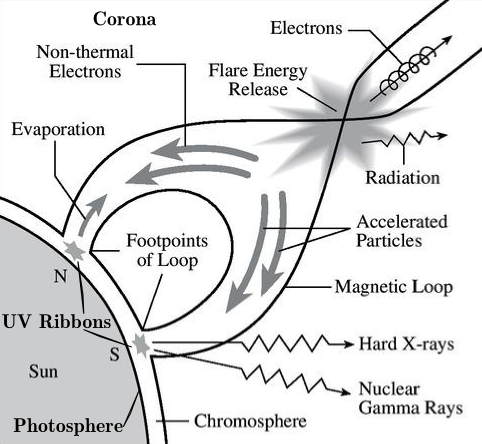
\includegraphics[width=0.40\textwidth]{flare}
  \caption{cartoon of the standard 2D solar flare model. Image courtesy of \href{http://ase.tufts.edu/cosmos/print_images.asp?id=47}{www.tufts.edu}}\label{flare-cartoon}
\end{center}
\end{figure}


%It is also theoretically possible to heat the upper photosphere by resistive dissipation of Alfven waves \citep{1982SoPh...80...99E}


\subsubsection{Solar Atmosphere}
The solar atmosphere is described as having four main components, the corona, transition region, chromosphere and photosphere, see Figure \ref{solatmpics}.

\begin{figure}[H]%\label{sunquake-cartoon}
  \begin{center}
  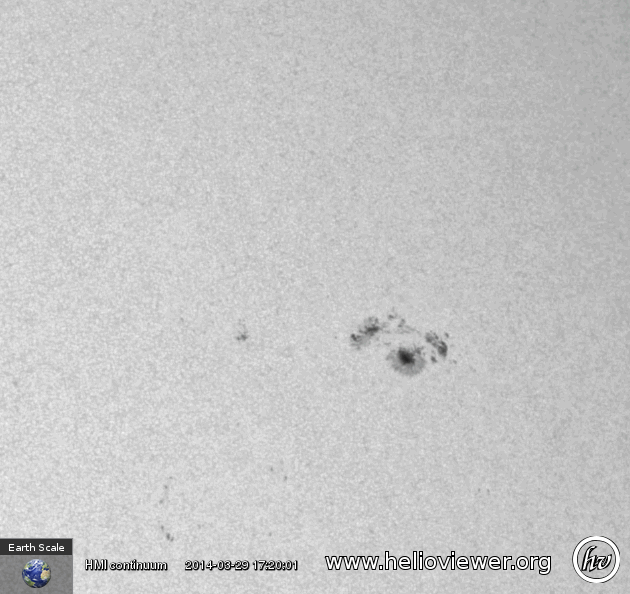
\includegraphics[width=0.20\textwidth]{2014_03_29_17_19_42_HMI_Int}%photsphere
  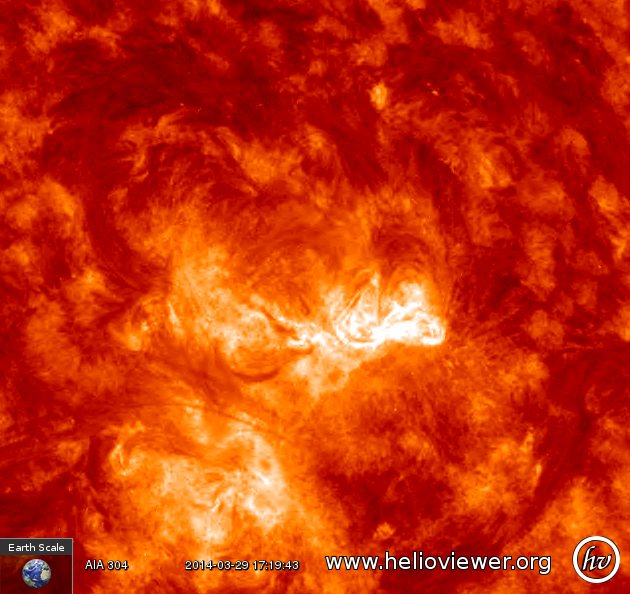
\includegraphics[width=0.20\textwidth]{2014_03_29_17_19_42_AIA_304}%chromosphere
  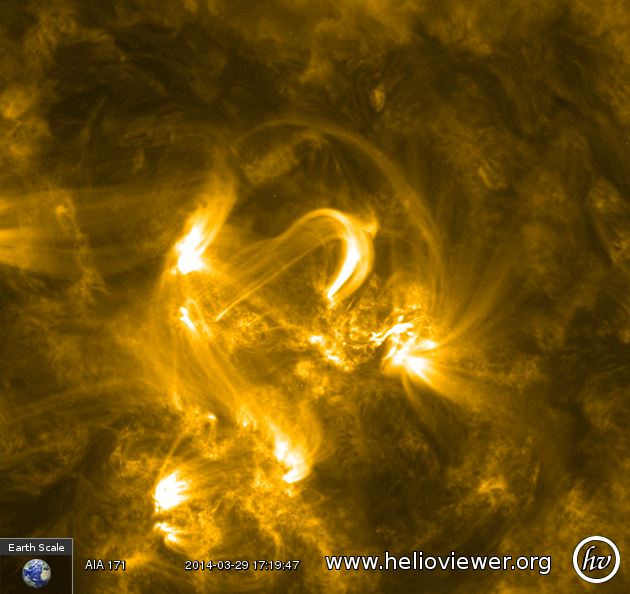
\includegraphics[width=0.20\textwidth]{2014_03_29_17_19_42_AIA_171}%tr
  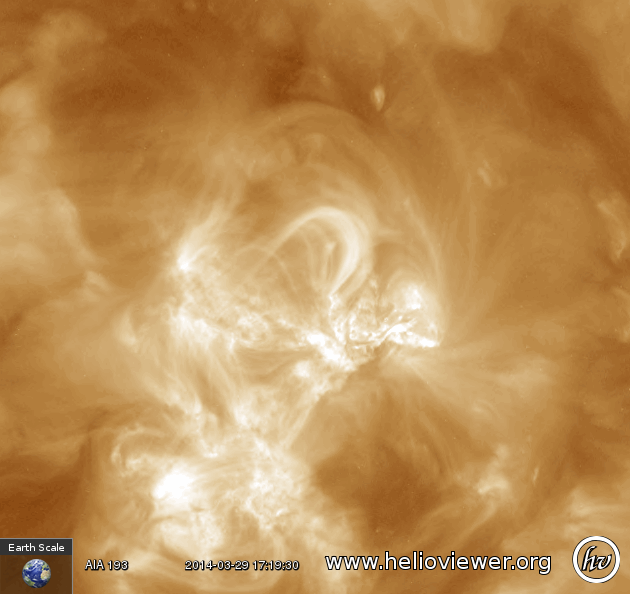
\includegraphics[width=0.20\textwidth]{2014_03_29_17_19_42_AIA_193}%corona
  \caption{ Images taken from the Solar Dynamics Observatory (SDO) instruments, the Helioseismic Magnetic Imager(HMI) and the Atmospheric Imaging Assembly (AIA) displaying the four main components of the solar atmosphere. From left to right layers of the solar atmosphere are increasing in altitude and temperature from the photosphere (SDO/HMI 6173 \AA\ continuum), to the chromosphere (SDO/AIA 304 \AA) through the transition region (SDO/AIA 171 \AA) then up to the corona (SDO/AIA 193 \AA). Images courtesy of \href{www.helioviewer.org}{www.helioviewer.org}}\label{solatmpics}
\end{center}
\end{figure}


For a sunquake to occur, energy released during a solar flare has to traverse these four layers propagating through nine pressure scale heights as it does so. Pressure scale height is a measure of the distance over which pressure drops off by a factor of \emph{e}. For example, in the photosphere, $H\sim150$km, whereas in the corona, $H\sim100$Mm. The photosphere is where sunquakes form observable wave-fronts and is the lowest in altitude of the four layers. With an effective temperature of $T=5800$K, the photosphere decreases in temperature with radial distance. If white light enhancement is observed in the photosphere, it is thought to be an indicator of the \textbf{Radiative backwarming} progenitor of sunquake generation, which can also be a bi-product caused by chromospheric \textbf{Shocks}. The plasma beta (a measure of the ratio between gas and magnetic pressure) in this region is mostly larger than one, $\beta >1$, meaning plasma pressure is dominant in dictating plasma motions, the exception to this exists in sunspots where $\beta<1$ and magnetic pressure is dominant. \\

Found in active regions of the photosphere, sunspots are regions of intense magnetic field playing host to footpoints of loops that can extend out into interplanetary space. They are made up of two main parts, the dark central umbra, surrounded by the slightly less dark penumbra. The umbra hosts magnetic field lines that are tightly packed and pointing radially away from the Sun, whereas the penumbral magnetic field is more horizontal with respect to the solar surface. During a solar flare, coronal loops reconnect causing a reconfiguration of the magnetic field tethered at sunspot locations, at this point, penumbral field lines can collapse toward the photosphere, imparting a Lorentz force on local plasma. This leads to the \textbf{Sudden magnetic field reconfiguration} progenitor of sunquake generation. Other features that are found on the photosphere include granules, which are the physical representation of convection currents. Heated plasma rises from below the surface and is seen as the bright central part of the granule, the darker surrounding regions are cooler material sinking back into the interior. \\

The next region of the atmosphere is the chromosphere which is situated above the photosphere. This layer of plasma is a few thousand kilometres (2000-3000km) thick and is optically thin to visible light so is difficult to see against the brightness of the photosphere. The temperature in this layer increases with height and ranges from 4400K at the temperature minimum region to $\sim10^{5}$K at the top, as a result, $\beta$ drops rapidly crossing unity as it does so. The pressure scale height in this region is changing with altitude. Through the transition region to the corona and the atmosphere starts to heat considerably to $T\sim10^{7}$K. This region is visible in white light due to Thompson scattering of photospheric light by free electrons and dust in the coronal magnetic field. The plasma beta is less than one through the entire corona meaning magnetic forces dominate. Figure \ref{solatm} shows how the solar atmosphere changes with height, temperature and density, giving an indication of the stratification of atmospheric layers. Information in this section is taken from text books: \cite{2003dysu.book.....D, 2004soas.book.....F}

\begin{figure}[H]
  \begin{center}
    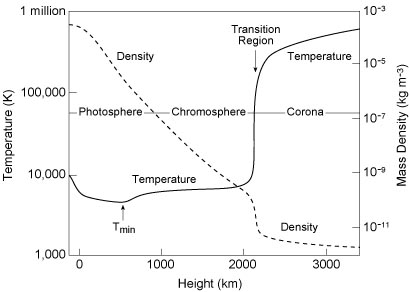
\includegraphics[width=0.6\textwidth]{solar-atm-plot}
\caption{The temperature of the solar atmosphere decreases from values near 6,000 degrees Kelvin at the visible photosphere to a minimum value of roughly 4,400 degrees Kelvin about 500 kilometres higher up. The temperature increases with height, slowly at first, then extremely rapidly in the narrow transition region, less than 100 kilometres thick, between the chromosphere and corona, from about $10^{4}$K to about $10^{6}$K. (Courtesy of Eugene Avrett, Smithsonian Astrophysical Observatory.)}\label{solatm}
  \end{center}
\end{figure}


\subsection{Observing Solar Flares}
Using data collected by spacecraft observing the Sun, energy released during solar flares can be tracked as it is deposited throughout the atmosphere. Energy deposition in the upper chromosphere is marked by HXR footpoints and UV ribbons. The Ramaty High Energy Solar Spectroscopic Imager (RHESSI) observes solar emission ranging from 1 keV X-rays to 20MeV $\gamma$-rays produced by energetic particles and nuclear interactions. RHESSI was designed with the aim of understanding impulsive energy release, particle acceleration and transportation in the magnetohydrodynamic environment of the solar atmosphere. Isolating the 10 - 100 keV energy data collected by RHESSI can provide information regarding the intensity and spatial origin of a HXR source. This allows the location of magnetic HXR footpoints to be tracked and the calculation of energy depostion by accelerated electrons.
\\
Observing UV ribbons requires a different spacecraft. The Interface Region Spectroscopic Imager (IRIS) captures near-ultraviolet (NUV) and far-ultraviolet (FUV) emission and is designed to observe the chromosphere at various altitudes. Emission is collected by a slit-jaw imager (SJI) and a spectrometer (SG) simultaneously. The spectrograph is sensitive in both FUV and NUV passbands, which expose 3 CCDs to produce spectra in three UV bands, two FUV and one NUV. Table \ref{iris-sg} shows how each passband relates to emission processes occurring from the upper-chromosphere down to the upper-photosphere.

\begin{table}[H]
\centering
\begin{tabular}{|c|c|c|c|}
Band & Wavelength \AA\ & Temperature $\log{T}$ & Region of Atmosphere\\
\hline
FUV 1 & $1331.7 - 1358.4$ & $3.7 - 7.0$ & Upper to lower-chromosphere\\
FUV 2 & $1389.0 - 1407.0$ & $3.7 - 5.2$ & Upper to lower-chromosphere\\
NUV & $2782.7 - 2851.1$ & $3.7 - 4.2$ & Chromosphere to upper-photosphere\\
\end{tabular}
\caption{The IRIS/SG is capable of observing three passbands, which relate to different plasma temperatures.}\label{iris-sg}
\end{table}

The slit-jaw images, are light collected from a reflective area surrounding the slit. The imager is capable of observing four wavelengths relating to emission at different altitudes as shown by Table \ref{iris-sj}.

\begin{table}[H]
\centering
\begin{tabular}{|c|c|c|c|c|}
SJI Passband & Wavelength \AA\ & FWHM \AA\ & Temperature $\log{T}$ & Region of Atmosphere\\
\hline
C II  & $1330$ & $40$ & $3.7 - 7.0$ & Upper-chromosphere\\
Si IV  & $1400$ & $40$ & $3.7 - 5.2$ & Upper-chromosphere\\
Mg II h/k & $2796$ & $4$ & $3.7 - 4.2$ & Lower-chromosphere\\
Mg II wing & $2832$ & $4$ & $3.7 - 3.8$ & Upper-photosphere\\
\end{tabular}
\caption{The IRIS/SJ is capable of observing four passbands, which relate to different plasma temperatures.}\label{iris-sj}
\end{table}

Signatures from energy deposition in the lowest regions of atmosphere are captured by Solar Dynamics Observatory's (SDO) Helioseismic Imager (HMI), which observes the photosphere. Able to observe optical continuum intensity (6173 \AA), helioseismic and magnetic data, SDO/HMI can provide valuable insight into WLFs, sunquakes and magnetic field configuration. Optical continuum data can provide information about WLFs and radiative backwarming of photospheric material, which is a possible sunquake progenitor. Helioseismic data can be used to analyse the movement of material during a solar flare, such as downward flows which could indicate shocks propagating from higher altitudes or particle beams penetrating the atmosphere. The point of origin and wave-fronts of a sunquake can also be detected using helioseismic data, which can be used to calculate acoustic power of the quake. Magnetic data from SDO/HMI shows local magnetic field direction, useful for determining the presence of impulsive changes in magnetic field capable of generating a sunquake.



%%%%%%%%%%%Observable Seismic Signatures%%%%%%%%%%%%%%%%%%%%%%%%%%
\subsection{Observable Seismic Signatures}
%Basics of helioseismology and challenges of observing acoustic emission
Helioseismology is a tool for probing the interior of the Sun. Most techniques in this field of analysis rely on observations of gravity and acoustic waves on the photosphere that are the result of interior excitation. Studying the frequency and modes of these oscillations has revealed much about the internal structure of the Sun. Local helioseismology is a collection of techniques developed for global helioseismology that have been modified for use in studying local regions in higher spatial resolution. The following section provides a very basic introduction to some of these techniques.

\subsubsection{Local Helioseismology}
%use content from old report...maybe expand a little

\paragraph{Helioseismic Holography}\label{helioholog}
\cite{1999ApJ...513L.143D} pioneered the use of helioseismic holography to produce seismic images of the solar flare of July 1996 reported to have a sunquake by Kosovichev and Zharkova. Time series egression-power maps at 3.5 and 6 mHz were computed with a 2 mHz bandwidth. It was found that the most powerful acoustic power frequency associated with the flare is centred at 3.5 mHz but has a large amount of noise. However, the 6 mHz range has a much lower ambient noise, therefore producing a better rendering of the seismicity of the flare. It is now standard practice to use the 6 mHz range for helioseismic holographic calculations of egression-power. \\
Originally the idea of analysing Doppler images of the solar surface in order to observe acoustic sources was put forward by \cite{1975CRASB.281...93R}. Helioseismic holography was developed further in concept by Lindsey and Braun \citep{1990SoPh..126..101L, 1992ApJ...392..739B, 1997ApJ...485..895L} in an effort to to image the solar interior and far-side of the Sun. This technique involves using a Doppler image of a location on the solar surface as a reference wave-field to enable an estimatation of that wave-field at a location in the solar interior at a time preceding or proceeding the image. This is achieved by calculating the ingression or egression of the wave-field by assuming that it's evolution is a, convergence to, or divergence from, the point of origin of that wave-field. The technique uses Green's function (eqn \ref{green}, where $\vec{r}$ and $t$ are position and time of an observed signal and $\vec{r}'$ and $t$' are the position and time of the signal earlier in time) which assumes that the acoustic wave propagates from a point source, allowing a signal $\psi(\vec{r},t)$ observed on the surface to be devolved backwards in time.

\begin{equation}\label{green}
G_{+}(|\vec{r}-\vec{r}'|,t-t')
\end{equation}

Where $a$ and $b$ constrain the holographic pupil, equation \ref{holog} is then used to devolve the surface signal to calculate the position of subsurface acoustic sources.

\begin{equation}\label{holog}
H_{+}(\vec{r},z,t)= \int dt'  \int_{a<|\vec{r}-\vec{r}'|<b} d^{2}\vec{r}'G_{+}(|\vec{r}-\vec{r}'|,t-t')\psi(\vec{r}',t')
\end{equation}

Equation \ref{eggpower} is then used to calculate the egression power associated with the acoustic sources at a time $t$.

\begin{equation}\label{eggpower}
P(z,\vec{r})=\int dt|H_{+}(\vec{r},z,t)|^{2}dt
\end{equation}

If egression power is required in terms of frequency then equation \ref{eggpower} can be Fourier transformed into frequency space.


\paragraph{Time-Distance}\label{TD}
The first observation of a sunquake \citep{1998Natur.393..317K} used the time-distance technique to track sunquake wavefronts. The paper by \cite{1993Natur.362..430D} explains how to extract time-distance (TD) information from observations of intensity fluctuations on the solar surface. This technique uses travel times of waves between two locations on the solar surface. The method assumes that the travel time of a wave propagating in the interior of the Sun will be modified by any anomalies that it has to travel through, thus the resulting signal will contain the signatures of those irregularities. For instance, if the wave encounters a flow along it's path of travel, it will propagate faster with the flow than against it, affecting travel time.
This technique remaps Dopplergrams into polar coordinates, with the point of origin centred on the area of downflowing material during the flare. This remapped image is then Fourier transformed with respect to azimuthal angle, with the resulting image highlighting circular disturbances as a line of positive slope.
